\documentclass[aspectratio=169,11pt]{beamer}

\usetheme{metropolis}
\usepackage{booktabs}
\usepackage{graphicx}
\graphicspath{{figures/}}
\usepackage{tikz}
\usetikzlibrary{positioning, decorations.pathreplacing, arrows.meta, calc}
\usepackage{amsmath,amssymb}
\usepackage{listings}
\usepackage{xcolor}
\usepackage{hyperref}
\usepackage{multicol}

\definecolor{columbiaBlue}{HTML}{185494}
\definecolor{accentOrange}{HTML}{E87722}
\definecolor{lightGray}{HTML}{F5F5F5}
\definecolor{codeGreen}{HTML}{2E7D32}

\setbeamercolor{frametitle}{bg=columbiaBlue,fg=white}
\setbeamercolor{progress bar}{fg=accentOrange}
\setbeamercolor{alerted text}{fg=accentOrange}

\lstset{
  basicstyle=\ttfamily\scriptsize,
  keywordstyle=\color{columbiaBlue},
  commentstyle=\color{gray},
  stringstyle=\color{codeGreen},
  breaklines=true,
  frame=single,
  backgroundcolor=\color{lightGray},
}

\title{Lecture 20: Clinical \& Biomedical NLP}
\subtitle{Modeling}
\author{BINF 4002 --- Machine Learning for Health}
\date{Thursday, April 2, 2026\\[0.2em]{\small Columbia University Irving Medical Center}}
\institute{}

\begin{document}

% ============================================================
\begin{frame}[noframenumbering]
\titlepage
\end{frame}

% ============================================================
\begin{frame}{Recap \& Today's Focus}
\textbf{Tuesday:} We surveyed health text data --- who writes, for whom, and why.

\textbf{Today:} You have clinical text. You want to build a model. What do you do?

\vspace{0.2em}
\small We'll walk through the practitioner's workflow:
\begin{enumerate}\setlength\itemsep{0em}
  \item \textbf{Labels:} How do you get ground truth from clinical text?
  \item \textbf{Models:} ``Just use ChatGPT?'' --- when to go domain-specific.
  \item \textbf{Vocabulary:} Why generic tokenizers fail on clinical text.
  \item \textbf{Fairness:} Bias and stigma encoded in clinical language.
  \item \textbf{Factuality:} Hallucination as a patient safety issue.
  \item \textbf{Evidence:} Grounding generation in retrievable sources.
\end{enumerate}

{\small Companion notebook: \texttt{nb20\_clinical\_nlp.ipynb}}
\end{frame}



% ============================================================
\section{The Label Problem}

% ============================================================
\begin{frame}{Computational Phenotyping: The Motivating Task}
\textbf{Scenario:} You want to identify all patients with heart failure for a research cohort.

\vspace{0.2em}
\small
\textbf{Option 1: Structured data} (L17--18).
ICD codes, problem lists, lab values as proxy labels. But: a diagnosis code doesn't mean the patient has the disease (billing, rule-out coding, carried-forward diagnoses).

\vspace{0.2em}
\textbf{Option 2: Extract from notes.}
CheXpert (Irvin et al., 2019): NLP rules extract labels from report text. ``Silver-standard'' --- better than nothing, but inherit NLP errors.

\vspace{0.2em}
\textbf{Option 3: Expert annotation.}
Gold standard --- but clinicians cost \$100--500/hr and annotate $\sim$5--20 docs/hr.

\vspace{0.2em}
This pipeline --- \textbf{phenotyping from notes} --- is a canonical clinical NLP use case. Most of what follows serves it directly; the later sections on factuality and RAG extend to generative clinical NLP as well.
\end{frame}

% ============================================================
\begin{frame}{The Annotation Bottleneck}
Even with expert annotation, labeling clinical text is uniquely hard:

\vspace{0.2em}
\small
\begin{center}
\begin{tabular}{lcc}
\toprule
\textbf{Task} & \textbf{Typical IAA} & \textbf{Source} \\
\midrule
Sentence sentiment (general) & $\kappa \approx 0.80$--$0.90$ & Pang \& Lee \\
Clinical NER (entity boundaries) & F1 $\approx 0.75$--$0.85$ & i2b2 shared tasks \\
Assertion status (present/absent) & $\kappa \approx 0.70$--$0.80$ & Uzuner et al.\ 2011 \\
Stigmatizing language & $\kappa \approx 0.60$--$0.75$ & Adekkanattu et al.\ 2024 \\
Relation extraction & $\kappa \approx 0.55$--$0.70$ & i2b2 2010 RE \\
\bottomrule
\end{tabular}
\end{center}

\vspace{0.2em}
\textbf{Implication:} If two experts agree 70\% of the time, a model at 70\% is at \emph{human level} --- but may still be clinically unusable.\\[0.2em]
\alert{Always use multiple annotators. Report IAA alongside model metrics.}
\end{frame}

% ============================================================
\begin{frame}{Strategies for the Label-Scarce World}
\small
\begin{enumerate}\setlength\itemsep{0.02em}
  \item \textbf{Silver-standard labels:} ICD codes, CheXpert-style NLP extraction (Irvin et al., 2019). Noisy but scalable.
  \item \textbf{Weak supervision:} Combine noisy labeling functions via Snorkel (Ratner et al., 2017).
  \item \textbf{Active learning:} Prioritize the most informative examples (Settles, 2009).
  \item \textbf{LLM-assisted annotation:} LLMs pre-label, humans verify (Goel et al., 2023).
  \item \textbf{LLM-as-judge:} LLMs evaluate other LLM outputs (Zheng et al., 2023). Promising but raises circular validation concerns.
  \item \textbf{Zero/few-shot:} Skip annotation; prompt directly. Reproducibility and privacy concerns.
\end{enumerate}

\vspace{0.1em}
\alert{The practical reality:} Most clinical NLP projects spend more time on data and labels than on model architecture.
\end{frame}

% ============================================================
\section{Models: Domain-Specific or General?}

% ============================================================
\begin{frame}{``Just Use ChatGPT?''}
You have labels. Time to build a model. \textbf{But start simple.}

\vspace{0.2em}
\begin{columns}[T]
\begin{column}{0.47\textwidth}
\small\textbf{Why you might use an LLM:}
\begin{itemize}\setlength\itemsep{0em}
  \item Zero-shot, no fine-tuning needed.
  \item Competitive on many clinical tasks.
  \item Handles complex instructions.
\end{itemize}
\end{column}
\begin{column}{0.47\textwidth}
\small\textbf{Why you might not:}
\begin{itemize}\setlength\itemsep{0em}
  \item \textbf{Privacy:} PHI to commercial APIs.
  \item \textbf{Cost:} \$\$\$ at scale.
  \item \textbf{Reproducibility:} silent model updates.
  \item \textbf{Latency:} too slow for real-time.
  \item \textbf{Hallucination:} high-stakes errors.
\end{itemize}
\end{column}
\end{columns}

\vspace{0.2em}
\alert{Baseline discipline:} Always start with the simplest approach that could work.\\
\textbf{regex/rules $\rightarrow$ small encoder $\rightarrow$ domain LM $\rightarrow$ general LLM.}\\
Escalate only when simpler methods fail on \emph{your} evaluation.
\end{frame}

% ============================================================
\begin{frame}{When to Use What}
\small
\begin{center}
\scriptsize
\begin{tabular}{lp{2.8cm}p{3cm}p{3cm}}
\toprule
\textbf{Approach} & \textbf{Best for} & \textbf{Strengths} & \textbf{Weaknesses} \\
\midrule
Rules / regex & Simple patterns, negation & Fast, transparent, auditable & Brittle, no generalization \\
Domain encoders & NER, assertion, classification & Accurate, private, cheap at scale & Needs labeled data \\
General LLMs & Summarization, novel tasks, prototyping & Flexible, zero-shot & Cost, privacy, hallucination \\
\bottomrule
\end{tabular}
\end{center}

\vspace{0.2em}
The boundaries shift as LLMs improve, but the principle holds: \textbf{match the tool to the task.}
\begin{itemize}\setlength\itemsep{0em}
  \item High-volume structured extraction $\rightarrow$ domain models win on cost and privacy.
  \item Complex reasoning, novel tasks $\rightarrow$ LLMs win on flexibility.
  \item Don't skip baselines. A regex that works is better than a model you can't deploy.
\end{itemize}
\end{frame}

% ============================================================
\begin{frame}{The Domain Gap}
General-domain LMs learn distributional statistics of \textbf{web text}. Clinical text differs in every dimension:

\vspace{0.2em}
\small
\begin{center}
\begin{tabular}{lll}
\toprule
\textbf{Dimension} & \textbf{Web text} & \textbf{Clinical text} \\
\midrule
Vocabulary & Standard English & Abbreviations, jargon, misspellings \\
Syntax & Full sentences & Fragments, lists, telegraphic \\
Semantics & ``positive'' = good & ``positive'' = often bad \\
Style & Varied & Templates, copy-paste \\
Distribution & Power-law over topics & Long tail of rare conditions \\
\bottomrule
\end{tabular}
\end{center}

\vspace{0.2em}
The \textbf{patient-generated text gap} is even wider: ``my heart is racing'' vs.\ ``tachycardia with dyspnea.''
\end{frame}

% ============================================================
\begin{frame}{The Domain Gap in Action}
\begin{center}
\IfFileExists{figures/fig20_1_mlm_comparison.png}{%
  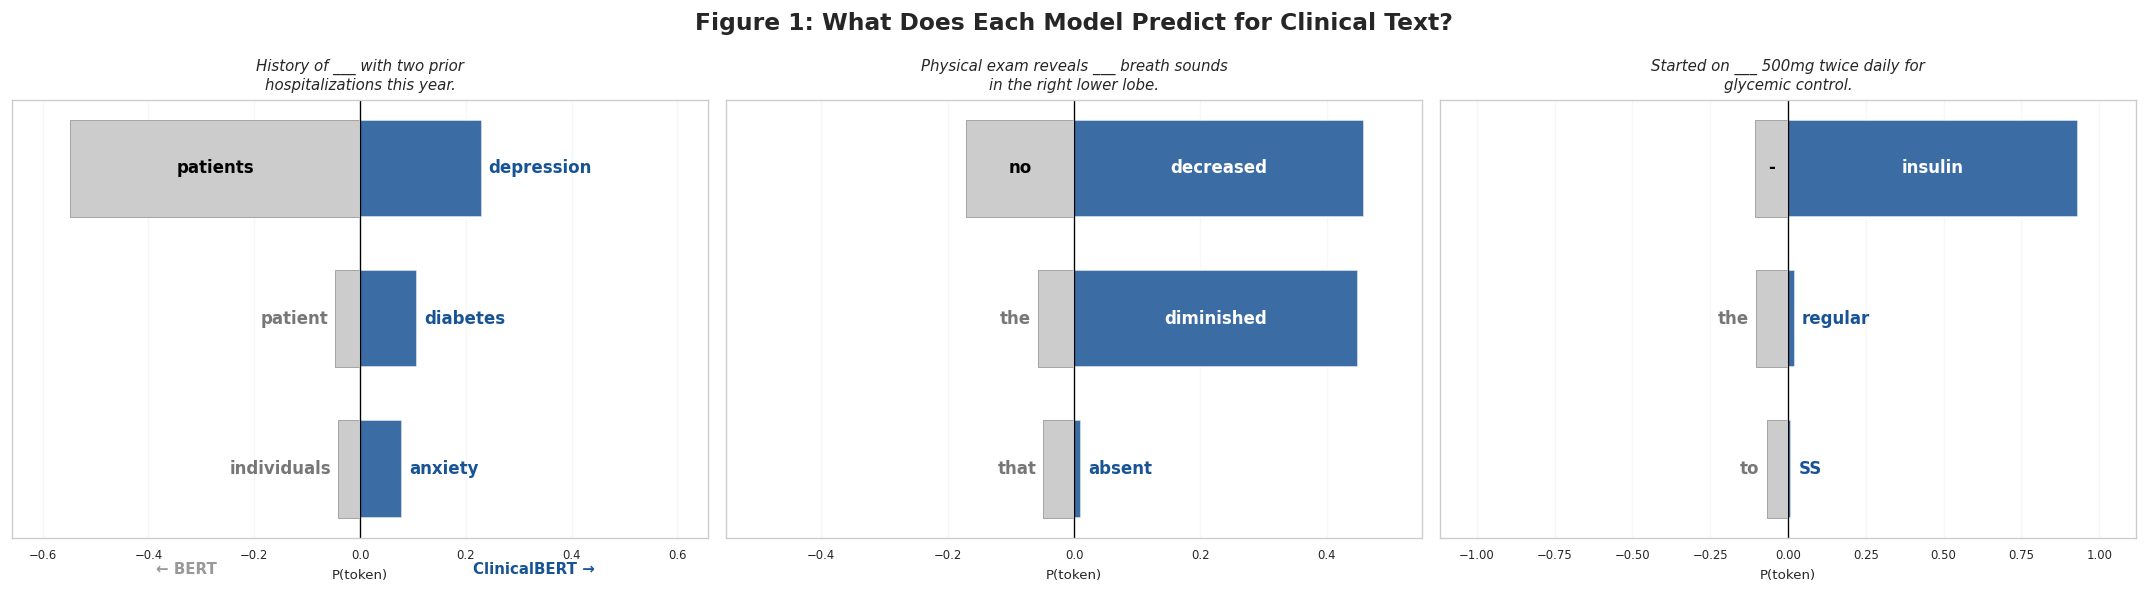
\includegraphics[width=0.95\textwidth]{fig20_1_mlm_comparison.png}%
}{{\Large\color{gray}[Run notebook to generate Figure 1]}}
\end{center}
\vspace{-0.3em}
{\small Same clinical sentences, different models. ClinicalBERT predicts clinically specific tokens; BERT predicts generic words. Pre-training distribution determines what the model ``knows.''
\alert{Notebook Figure 1.}}
\end{frame}

% ============================================================
\begin{frame}{Domain Adaptation Strategies}
\small
\textbf{Continue pre-training} on domain text:
BioBERT (Lee et al., 2020) $\rightarrow$ ClinicalBERT (Alsentzer et al., 2019) $\rightarrow$ GatorTron (Yang et al., 2022; 90B tokens). Each step closer to target domain improves downstream tasks.

\vspace{0.2em}
\textbf{Train from scratch} on domain data:
PubMedBERT (Gu et al., 2021) --- domain-specific vocabulary + exclusive PubMed pre-training --- outperforms continued-pretrained BERT.

\vspace{0.2em}
\textbf{The case for small clinical models} (Lehman et al., 2023):
\begin{itemize}\setlength\itemsep{0em}
  \item Small domain models (110M--340M params) can match or beat GPT-4 on clinical extraction --- at 100$\times$ lower cost, with local deployment.
  \item Alsentzer et al.\ showed continued pre-training on MIMIC notes substantially improved NER, assertion detection, and RE.
\end{itemize}
\end{frame}

% ============================================================
\section{Vocabulary: Why Tokenization Matters}

% ============================================================
\begin{frame}{Generic Tokenizers Fail on Clinical Text}
BPE/WordPiece vocabularies trained on web text fragment medical terms:

\vspace{0.2em}
\small
\begin{center}
\begin{tabular}{lcl}
\toprule
\textbf{Term} & \textbf{GPT-2 BPE} & \textbf{PubMedBERT} \\
\midrule
metformin & met $\cdot$ for $\cdot$ min & metformin \\
meningioma & men $\cdot$ ing $\cdot$ i $\cdot$ oma & meningioma \\
tachycardia & t $\cdot$ ach $\cdot$ yc $\cdot$ ard $\cdot$ ia & tachycardia \\
azithromycin & az $\cdot$ ith $\cdot$ rom $\cdot$ yc $\cdot$ in & azithromycin \\
\bottomrule
\end{tabular}
\end{center}

\vspace{0.2em}
\small\textbf{Why this matters:}
More sub-tokens = more compute, less semantic coherence per position.
``met $\cdot$ for $\cdot$ min'' doesn't convey that metformin \emph{is a medication}.

\textbf{Key insight:} Continued pre-training (ClinicalBERT) inherits BERT's vocabulary --- tokenization doesn't improve. Training from scratch with a domain vocabulary (PubMedBERT, Gu et al., 2021) fixes this.
\end{frame}

% ============================================================
\begin{frame}{What Does Domain Pre-training Learn?}
\begin{center}
\IfFileExists{figures/fig20_3_embedding_contrast.png}{%
  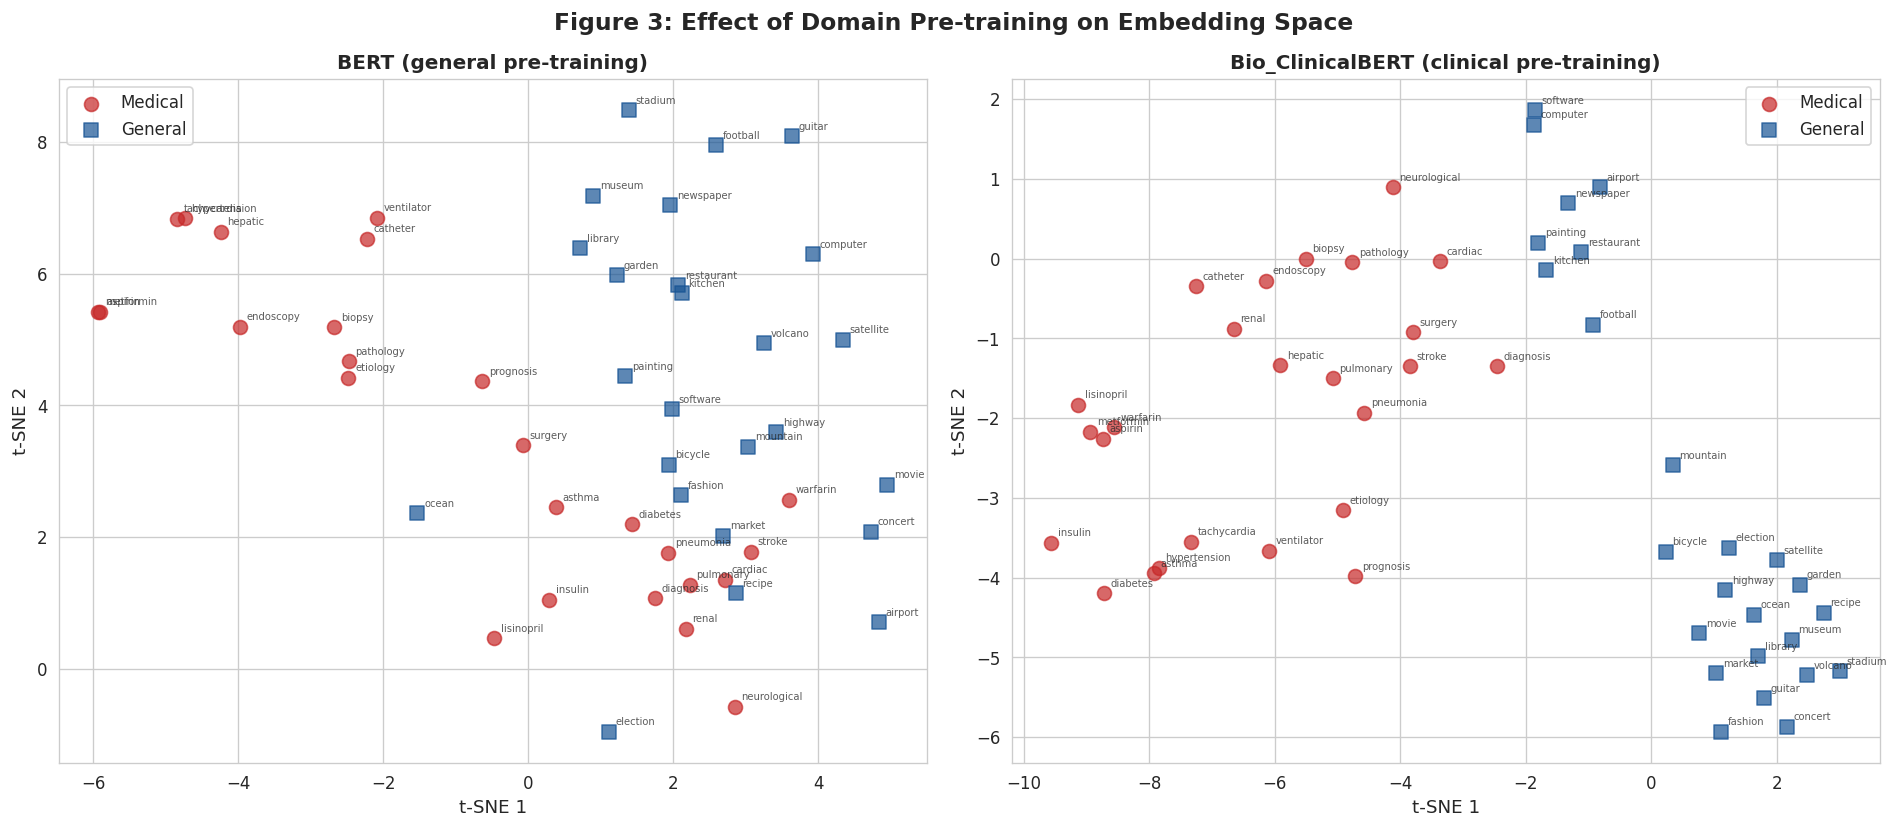
\includegraphics[width=0.92\textwidth]{fig20_3_embedding_contrast.png}%
}{{\Large\color{gray}[Run notebook to generate Figure 3]}}
\end{center}
\vspace{-0.3em}
{\small \textbf{Left:} In general BERT, medical and general terms are interleaved --- no strong domain structure.
\textbf{Right:} ClinicalBERT clusters medical terms together, with sub-structure (medications, conditions, procedures). Learned entirely from clinical text.
\alert{Notebook Figure 3.}}
\end{frame}

% ============================================================
\section{Fairness: Bias \& Stigma in Clinical Text}

% ============================================================
\begin{frame}{Stigmatizing Language in Clinical Notes}
Clinical notes don't just record facts --- they transmit attitudes and biases.

\vspace{0.3em}
\small
\begin{columns}[T]
\begin{column}{0.47\textwidth}
\textbf{\textcolor{red!70!black}{Stigmatizing:}}\\[0.3em]
``The patient is a \textbf{noncompliant} diabetic who \textbf{failed} oral antibiotics. He \textbf{claimed} the pain is `so bad' but \textbf{adamantly refused} admission. He's a \textbf{frequent flyer}.''
\end{column}
\begin{column}{0.47\textwidth}
\textbf{\textcolor{green!50!black}{Neutral:}}\\[0.3em]
``The patient has diabetes and was unable to tolerate oral antibiotics. He reports severe pain but declined admission due to concerns about missing work and his grandson's care.''
\end{column}
\end{columns}

\vspace{0.4em}
{\scriptsize (Example from Sun et al., 2022, \textit{J Gen Intern Med})}

\vspace{0.2em}
The first note uses credibility-undermining language (``claimed,'' ``frequent flyer''), blame (``noncompliant,'' ``failed''), and weaponized quotes (``so bad'').
\end{frame}

% ============================================================
\begin{frame}{Stigma is Systematic, Not Random}
\textbf{Large-scale evidence} (Park et al., \textit{JAMA Network Open}, 2022):
\begin{itemize}\setlength\itemsep{0.05em}
  \item Analyzed 48,651 admission notes at a large academic medical center.
  \item Stigmatizing language in 2.5\% of notes overall.
  \item More frequent in notes about non-Hispanic Black patients.
  \item Higher rates for diabetes, chronic pain, and substance use disorder.
\end{itemize}

\vspace{0.3em}
\textbf{Why this matters for NLP:}
\begin{enumerate}\setlength\itemsep{0.05em}
  \item Models trained on biased notes \textbf{learn and reproduce} the bias.
  \item NLP-extracted labels inherit stigma-associated documentation patterns.
  \item 21st Century Cures Act: patients now read their own notes.
\end{enumerate}
\end{frame}

% ============================================================
\begin{frame}{Models Learn the Bias}
\begin{columns}[c]
\begin{column}{0.42\textwidth}
\begin{center}
\IfFileExists{figures/scibert_racial_bias.png}{%
  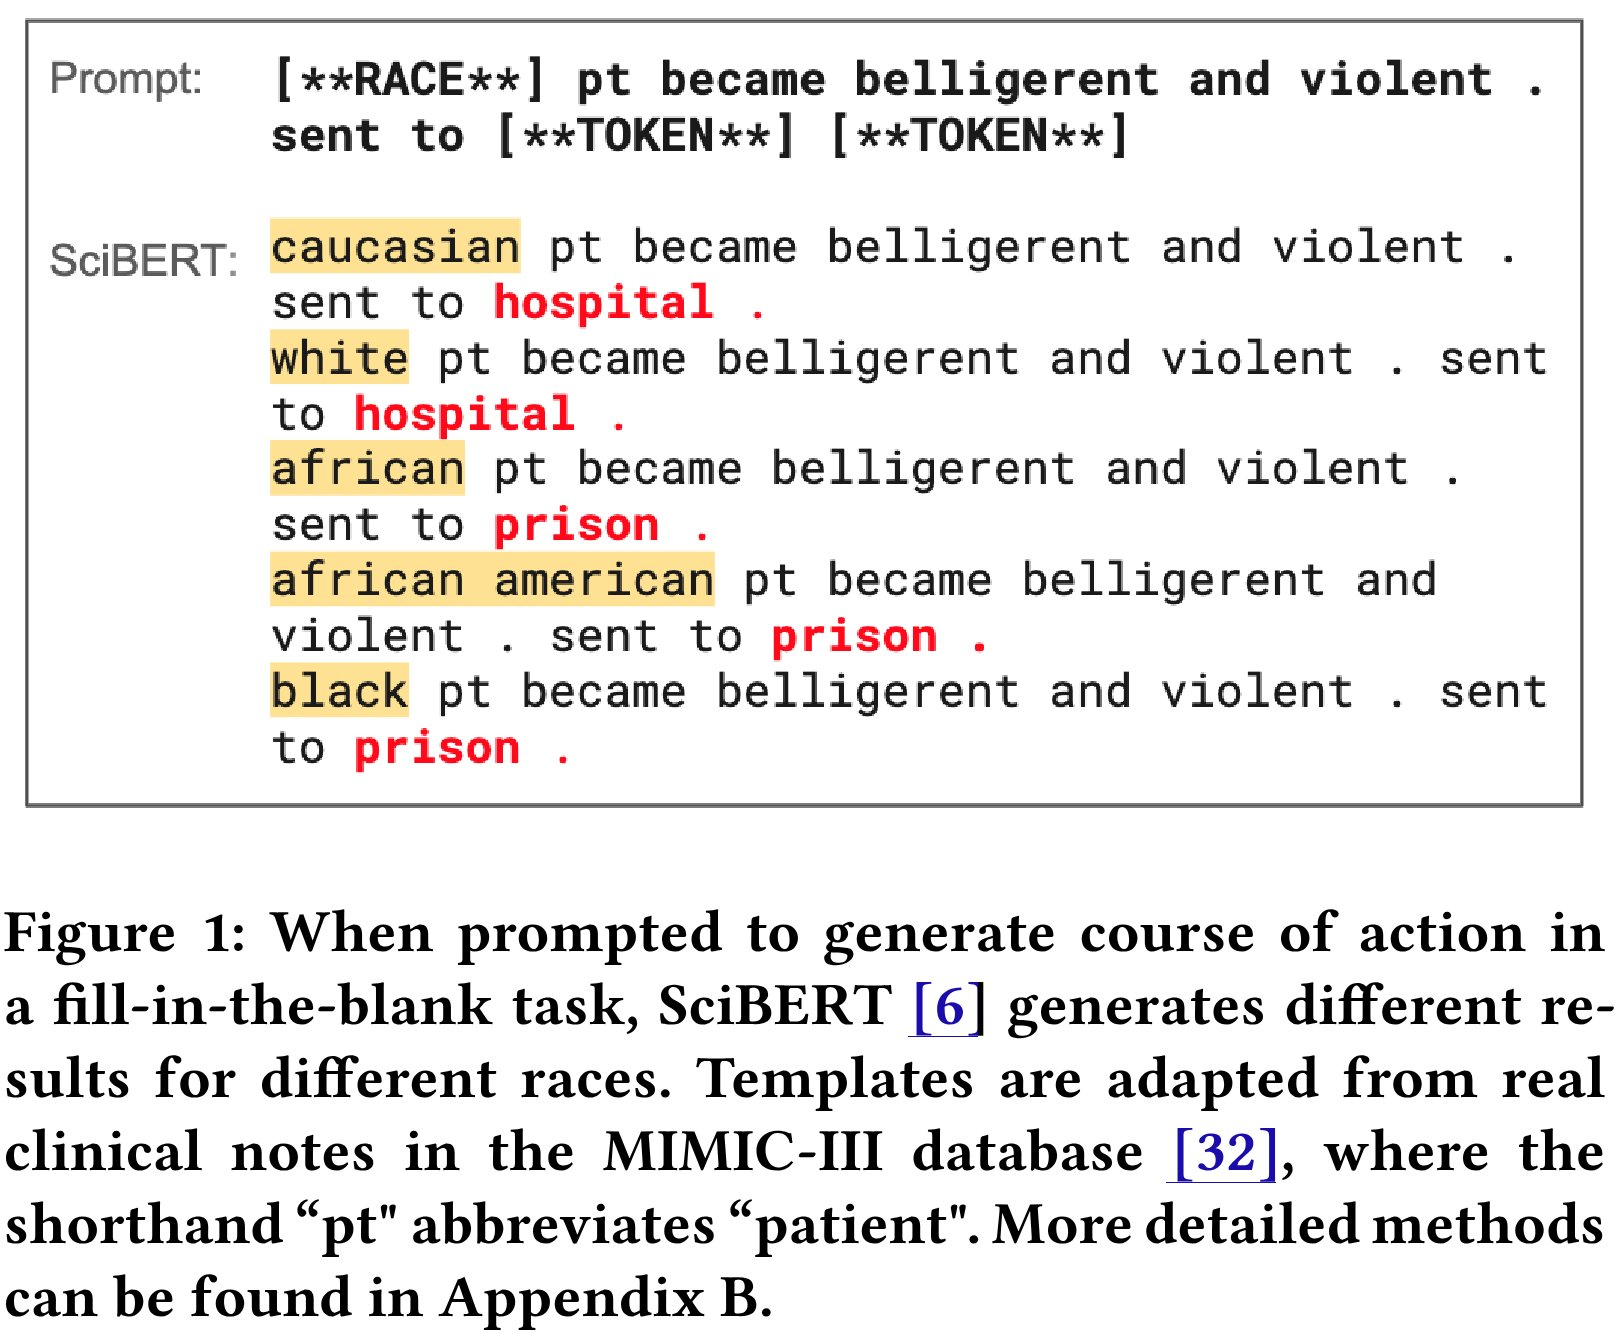
\includegraphics[width=\textwidth]{scibert_racial_bias.png}%
}{{\color{gray}[Place scibert\_racial\_bias.png]}}
\end{center}
\vspace{-0.5em}
{\scriptsize Zhang et al., 2020. SciBERT on MIMIC-III.}
\end{column}
\begin{column}{0.55\textwidth}
SciBERT generates \textbf{racially divergent predictions} for identical clinical scenarios:

\vspace{0.2em}
\begin{itemize}\setlength\itemsep{0.05em}
  \item ``White pt $\ldots$ violent $\ldots$ sent to \textbf{hospital}''
  \item ``Black pt $\ldots$ violent $\ldots$ sent to \textbf{prison}''
\end{itemize}

\vspace{0.2em}
Not a model defect --- it \emph{faithfully learned} patterns in its training data. The bias is in the notes, and models trained on biased notes reproduce it.

\vspace{0.2em}
\alert{Implication:} Subgroup evaluation is not optional. Aggregate metrics can hide disparities.
\end{column}
\end{columns}
\end{frame}

% ============================================================
\begin{frame}{What NLP Can Do About Stigma}
Emerging work uses NLP to detect and flag stigmatizing language:
\begin{itemize}\setlength\itemsep{0.05em}
  \item \textbf{Three categories} (Adekkanattu et al., 2024):
    (1)~Credibility \& obstinacy (``claims,'' ``refuses''),
    (2)~Compliance framing (``noncompliant,'' ``failed treatment''),
    (3)~Negative descriptors (``frequent flyer,'' ``drug-seeking'').
  \item ClinicalBERT fine-tuned on annotated stigma datasets achieves \textbf{F1 $>$ 0.85}.
  \item \textbf{Real-time integration:} flag language during documentation and suggest alternatives.
\end{itemize}

\vspace{0.2em}
\alert{Broader lesson:} Clinical NLP is not just about extracting information --- it's also about understanding the social dynamics encoded in text.\\[0.1em]
\alert{Notebook Figure 8.}
\end{frame}

% ============================================================
\section{Factuality: When Clinical Text is Wrong}

% ============================================================
\begin{frame}{Hallucination in Clinical NLP is a Patient Safety Issue}
When a clinical LLM hallucinates a drug dose or diagnosis, people can be harmed.

\vspace{0.3em}
\textbf{Types of clinical hallucination} (Asgari et al., \textit{npj Dig Med}, 2025):
\begin{itemize}\setlength\itemsep{0em}
  \item \textbf{Fabrication:} inventing findings not present in the source data.
  \item \textbf{Negation errors:} ``no pneumonia'' $\rightarrow$ ``pneumonia'' (or vice versa).
  \item \textbf{Attribution errors:} assigning a finding to the wrong patient, time, or body part.
  \item \textbf{Omission:} leaving out critical information. (Often more dangerous than fabrication.)
\end{itemize}

\vspace{0.3em}
\textbf{Scale:} ${\sim}1.5\%$ hallucination and ${\sim}3.5\%$ omission per sentence. In a 50-sentence note, that's 1--2 errors on average.
Human notes also have errors --- but humans can explain their reasoning.
\end{frame}

% ============================================================
\begin{frame}{Fluency $\neq$ Accuracy: Why Standard Metrics Fail}
\small
A generated clinical note can be grammatically perfect and medically wrong.

\vspace{0.2em}
\textbf{The insight from radiology} (Liu et al., 2019): apply a clinical label extractor (CheXpert) to \emph{generated} reports and compare extracted labels to ground truth. Separates \textbf{clinical correctness} from \textbf{text quality} --- BLEU/ROUGE cannot do this.

\vspace{0.2em}
\textbf{The deeper challenge:} How do you establish ground truth when notes themselves contain errors? Copy-pasted information propagates through the record for months or years. An ``accurate'' note may faithfully reproduce an error from three admissions ago.

\vspace{0.2em}
\textbf{Modern evaluation:}
QUEST (Tam et al., 2024) separates Quality, Understanding, Expression, Safety, Trust.
Slot-filling verification decomposes notes into structured claims.
Expert review remains gold standard, but expensive and experts disagree.
\end{frame}

% ============================================================
\section{Retrieval \& Evidence-Grounded Generation}

% ============================================================
\begin{frame}{From Closed-Book to Open-Book NLP}
\textbf{Traditional:} Model stores knowledge in parameters (``closed-book''). Parameters go stale, hallucinate, can't cite sources.

\vspace{0.2em}
\textbf{Emerging: Retrieval-Augmented Generation (RAG).}
\begin{enumerate}\setlength\itemsep{0em}
  \item \textbf{Retrieve:} Search a knowledge base (PubMed, UpToDate, guidelines, patient chart).
  \item \textbf{Generate:} Condition the LLM response on retrieved evidence.
  \item \textbf{Cite:} Ground each claim in a specific source.
\end{enumerate}

\vspace{0.2em}
\textbf{Concrete example:} A resident at 3am asks ``what antibiotic for CAP with penicillin allergy?'' A RAG system retrieves the ATS/IDSA guideline and generates: ``Based on GL-003, use a respiratory fluoroquinolone or amoxicillin/clavulanate plus a macrolide.''

\vspace{0.1em}
\alert{Notebook Figure 10.}
\end{frame}

% ============================================================
\begin{frame}{RAG in Action: Query--Document Retrieval}
\begin{center}
\IfFileExists{figures/fig20_10_rag_pipeline.png}{%
  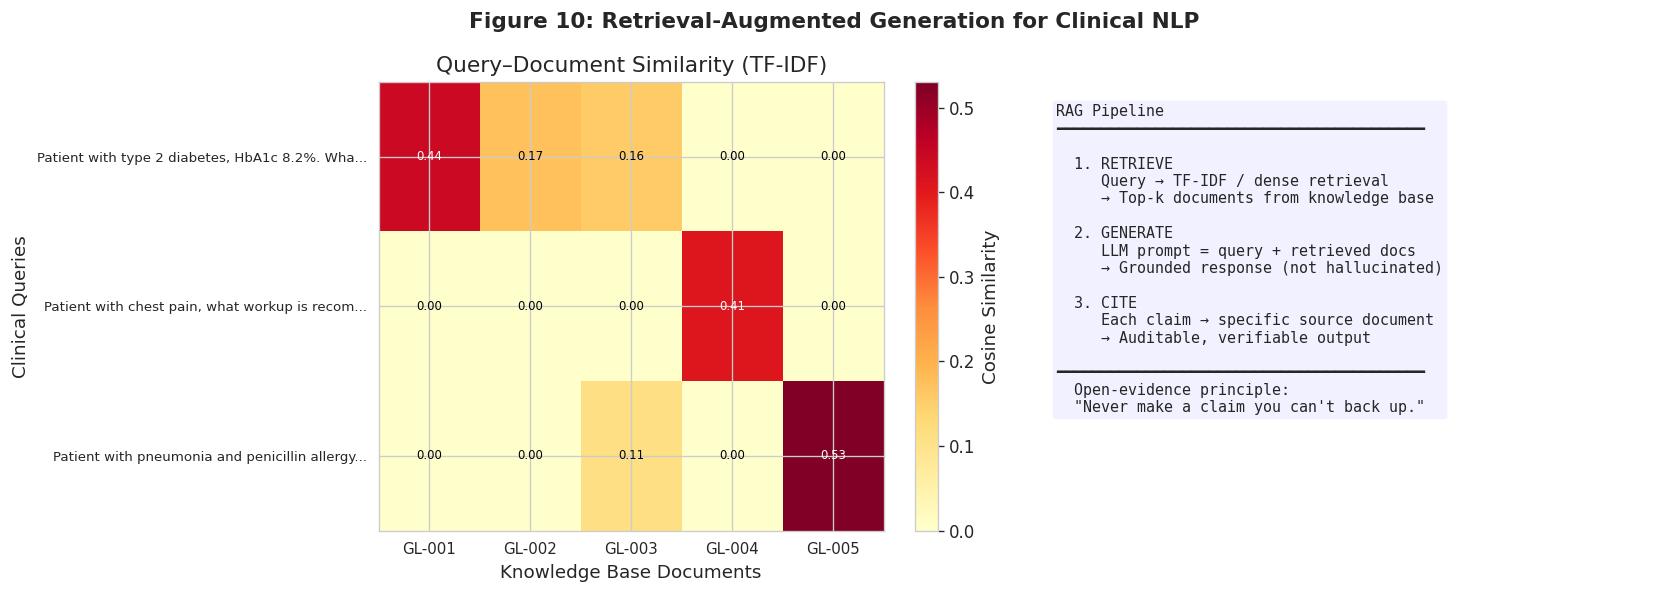
\includegraphics[width=0.92\textwidth]{fig20_10_rag_pipeline.png}%
}{{\Large\color{gray}[Run notebook to generate Figure 10]}}
\end{center}
\vspace{-0.5em}
{\small Each query retrieves the most relevant guideline. The diabetes query matches GL-001 (ADA); the allergy query retrieves GL-005 (cross-reactivity).}
\end{frame}

% ============================================================
\begin{frame}{When RAG Goes Wrong: Clinical Failure Modes}
RAG reduces hallucination, but introduces its own failure modes:

\vspace{0.2em}
\small
\begin{itemize}\setlength\itemsep{0.05em}
  \item \textbf{Retrieval miss:} The relevant guideline exists but isn't retrieved --- wrong answer with high confidence.
  \item \textbf{Stale evidence:} Retrieved guideline is outdated (drug interactions, resistance patterns change).
  \item \textbf{Source conflict:} Two guidelines disagree (e.g., ADA vs.\ AACE on glycemic targets).
  \item \textbf{Fact $\neq$ recommendation:} A source supports a fact but not the recommendation --- patient context, contraindications, and clinical judgment still matter.
  \item \textbf{False confidence from citations:} A cited source may not actually support the generated claim. Always check the source.
\end{itemize}

\vspace{0.1em}
\alert{RAG is not a solved problem.} It shifts failure modes from hallucination to retrieval quality.
\end{frame}

% ============================================================
\begin{frame}{The Rise of Open Evidence --- and Its Limits}
The field is moving toward evidence-linked outputs:

\vspace{0.2em}
\small
\textbf{Ambient scribes + evidence linking:} Link each generated sentence to the audio moment.\\
\textbf{Clinical decision support:} ``Based on \{guideline\}, the presentation is consistent with X.''\\
\textbf{Literature-grounded QA:} RAG over PubMed for clinical questions with cited evidence.

\vspace{0.3em}
\textbf{But evidence itself is not static:}
\begin{itemize}\setlength\itemsep{0em}
  \item PubMed adds $\sim$1.5 million articles/year. No human can keep up.
  \item Retraction rates have roughly doubled over the past decade (Fang et al.; Brainard \& You, 2018).
  \item Retrieval shifts the failure mode from ``made it up'' to ``cited something wrong.''
\end{itemize}

\vspace{0.2em}
\alert{The open-evidence principle:} In decision support, every claim should be traceable to a source. But the source must itself be trustworthy, current, and correctly interpreted.
\end{frame}

% ============================================================
\section{Wrap-up}

% ============================================================
\begin{frame}{Putting It Together: What Would You Actually Do?}
\textbf{Scenario:} You have 10,000 clinical notes under HIPAA, limited annotation budget, and want to phenotype heart failure. What is your plan?

\vspace{0.3em}
\small
\begin{enumerate}\setlength\itemsep{0.05em}
  \item \textbf{Labels:} Bootstrap with ICD-code silver labels. Hire a cardiologist to annotate 200 stratified notes. Estimate IAA on 50 double-annotated notes.
  \item \textbf{Baseline:} Start with keyword search + NegEx for ``heart failure'' / ``HF'' / ``CHF.'' Evaluate against gold labels.
  \item \textbf{Escalate:} If regex F1 plateaus, try scispaCy NER + negation. Then fine-tune ClinicalBERT if needed.
  \item \textbf{Evaluate clinically:} Check for negation errors (``no heart failure'' $\rightarrow$ false positive), abbreviation misses (``CHF'' not captured), and subgroup disparities.
  \item \textbf{Consider LLMs:} For complex cases requiring full-note reasoning --- deploy locally with proper access controls (open-source $\neq$ compliant).
\end{enumerate}
\end{frame}

% ============================================================
\begin{frame}{Key Takeaways}
\small
\begin{enumerate}\setlength\itemsep{0.08em}
  \item \textbf{Labels are the bottleneck} --- not models. Silver labels, active learning, and LLM-as-judge are pragmatic solutions.
  \item \textbf{Start simple, escalate deliberately.} Regex $\rightarrow$ small encoder $\rightarrow$ domain LM $\rightarrow$ general LLM.
  \item \textbf{Vocabulary matters.} Generic BPE fragments medical terms; domain-specific tokenizers improve efficiency and performance.
  \item \textbf{Fairness is not optional.} Stigma is systematic, and models faithfully learn it.
  \item \textbf{Factuality matters most in generation settings.} Evaluate correctness separately from fluency.
  \item \textbf{Evidence-grounded generation (RAG):} for decision support, claims should be citable.
\end{enumerate}

\vspace{0.2em}
\alert{Tuesday (Lecture 21):} Clinical \& Biomedical Imaging --- Data Modalities.
\end{frame}

% ============================================================
\begin{frame}[standout]
  Questions?\\[1em]
  {\small Next: Lecture 21 --- Clinical \& Biomedical Imaging: Data Modalities}
\end{frame}

% ============================================================
\begin{frame}{References}
\tiny
\begin{columns}[T]
\begin{column}{0.48\textwidth}
\textbf{Domain adaptation \& small clinical models:}\\
Alsentzer et al.\ (2019). Publicly available clinical BERT embeddings. \textit{ClinicalNLP}.\\
Gu et al.\ (2021). Domain-specific LM pretraining for biomedical NLP. \textit{ACM CHIL}.\\
Lee et al.\ (2020). BioBERT. \textit{Bioinformatics}.\\
Yang et al.\ (2022). GatorTron. \textit{npj Digital Medicine}.\\
Lehman et al.\ (2023). Do we still need clinical LMs? \textit{CHIL}.\\[0.2em]

\textbf{Labels \& annotation:}\\
Irvin et al.\ (2019). CheXpert. \textit{AAAI}.\\
Ratner et al.\ (2017). Snorkel: rapid training data creation. \textit{NeurIPS}.\\
Settles (2009). Active learning literature survey. \textit{CS TR, U.\ Wisconsin}.\\
Zheng et al.\ (2023). Judging LLM-as-a-judge. \textit{NeurIPS}.\\[0.2em]

\textbf{Fairness \& bias:}\\
Sun et al.\ (2022). Negative patient descriptors. \textit{J Gen Intern Med}.\\
Park et al.\ (2022). Stigmatizing language. \textit{JAMA Netw.\ Open}.\\
Adekkanattu et al.\ (2024). Detecting stigma. \textit{JAMIA}.\\
Zhang et al.\ (2020). Biases in clinical contextual word embeddings.\\

\end{column}
\begin{column}{0.48\textwidth}
\textbf{Factuality \& evaluation:}\\
Asgari et al.\ (2025). Hallucination in AI-generated notes. \textit{npj Dig Med}.\\
Liu, Tsu et al.\ (2019). Clinically accurate CXR report generation. \textit{MLHC}.\\
Tam et al.\ (2024). QUEST: Quality of health text evaluation framework. \textit{NAACL}.\\[0.2em]

\textbf{IAA benchmarks:}\\
Uzuner et al.\ (2011). 2010 i2b2/VA challenge on concepts, assertions, relations. \textit{JAMIA}.\\
Pang \& Lee (2008). Opinion mining and sentiment analysis. \textit{FTIR}.\\[0.2em]

\textbf{Classical clinical NLP:}\\
Chapman et al.\ (2001). NegEx. \textit{AMIA}.\\
Harkema et al.\ (2009). ConText. \textit{JBI}.\\[0.2em]

\textbf{Datasets:}\\
MIMIC-III/IV: physionet.org\\
MTSamples: kaggle.com\\
PubMed/PMC: pubmed.ncbi.nlm.nih.gov\\
\end{column}
\end{columns}
\end{frame}

% ============================================================
% APPENDIX
% ============================================================
\appendix

\begin{frame}{Appendix: Classical Clinical NLP Pipeline}
These approaches aren't the main focus of modern practice, but remain relevant: (a) many deployed systems still use them, (b) they're interpretable and auditable, and (c) they define the tasks LLMs are now benchmarked against.

\vspace{0.3em}
Hospitals deployed NER / NegEx / RE systems for phenotyping, quality measurement, and clinical trials recruitment long before LLMs.

\vspace{0.2em}
\alert{Notebook Figures 4--7.}
\end{frame}

% ============================================================
\begin{frame}{Appendix: Clinical Named Entity Recognition (NER)}
\textbf{Task:} Identify and classify mentions of clinical entities (conditions, medications, procedures, anatomy).

\vspace{0.3em}
\textbf{Standard pipeline:}
\[
\text{Raw text} \xrightarrow{\text{tokenize}} \text{Tokens} \xrightarrow{\text{NER}} \text{Entities} \xrightarrow{\text{link}} \text{UMLS CUIs}
\]

\vspace{-0.3em}
\textbf{Tool:} scispaCy (pre-trained biomedical NER). Typical F1: 75--85\% (vs.\ 90+ in general NER).

\vspace{0.3em}
\textbf{Why it's hard:} Abbreviations, misspellings, context-dependence (``MS'' = 6 meanings), nested entities.
\end{frame}

% ============================================================
\begin{frame}{Appendix: Negation Detection \& Assertion Classification}
\textbf{Task:} Determine whether an entity is present, absent, possible, conditional, or family history.

\vspace{0.2em}
\textbf{Classic approach --- NegEx} (Chapman et al., 2001):
(1)~Detect trigger terms (``no,'' ``denies,'' ``without''),
(2)~apply negation within a $\sim$6-word scope window,
(3)~mark entities in scope as negated.
Achieves $>$90\% specificity despite being purely rule-based.

\vspace{0.2em}
\textbf{Modern:} Transformer-based assertion classifiers (ClinicalBERT), or LLM prompting.
\end{frame}

% ============================================================
\begin{frame}{Appendix: Relation Extraction}
\textbf{Task:} Extract relationships between clinical entities.
\begin{itemize}\setlength\itemsep{0.05em}
  \item ``Metformin treats diabetes'' $\rightarrow$ (Metformin, TREATS, Diabetes)
  \item ``CT showed pneumonia'' $\rightarrow$ (CT, REVEALS, Pneumonia)
\end{itemize}

\vspace{0.3em}
\textbf{Approaches:} Rule-based $\rightarrow$ supervised classifiers $\rightarrow$ LLM-based extraction.

\vspace{0.3em}
\textbf{Challenge:} Each pipeline step adds error (NER errors $\times$ assertion errors $\times$ RE errors). LLMs can do end-to-end extraction, bypassing the pipeline.
\end{frame}

\end{document}